\documentclass[a4paper,10pt]{article}
\usepackage[paper=a4paper, hmargin=1.5cm, bottom=1.5cm, top=3.5cm]{geometry}
\usepackage[utf8]{inputenc} %Codificacion de caracteres, para poder usar acentos, etc.
\usepackage[T1]{fontenc}
\usepackage[spanish]{babel}
\usepackage{xspace}
\usepackage{xargs} %Para crear funciones con muchos argumentos
\usepackage{ifthen}
\usepackage{aed2-tad,aed2-symb,aed2-itef,caratula} %Macros de Algo2
\usepackage{algorithm}% http://ctan.org/pkg/algorithms
\usepackage{algpseudocode} % Para algorritmia
%\usepackage{algorithmic} %paquete para hacer pseudocodigo

\usepackage{titlesec}%http://foro-c.com/blog/latex-formato-de-titulos-de-capitulos-secciones-etc/
\usepackage{graphicx} %Inlcuir imagenes.
\usepackage{setspace}
\usepackage{fancyhdr}
\usepackage[colorlinks=true, linkcolor=blue]{hyperref} %Links para el indice.
\usepackage{float} %Insercion de imagenes flotantes
\usepackage{ stmaryrd }

\usepackage{caption}
\usepackage{subcaption}

\newcommand{\moduloNombre}[1]{\textbf{#1}}

\let\NombreFuncion=\textsc
\let\TipoVariable=\texttt
\let\ModificadorArgumento=\textbf
\newcommand{\res}{$res$\xspace}
\newcommand{\tab}{\hspace*{7mm}}

\newcommandx{\TipoFuncion}[3]{%
  \NombreFuncion{#1}(#2) \ifx#3\empty\else $\to$ \res\,: \TipoVariable{#3}\fi% nombreFuncion(parametros) -> res:(Tipo)
}
\newcommand{\In}[2]{\ModificadorArgumento{in} \ensuremath{#1}\,: \TipoVariable{#2}\xspace}
\newcommand{\Out}[2]{\ModificadorArgumento{out} \ensuremath{#1}\,: \TipoVariable{#2}\xspace}
\newcommand{\Inout}[2]{\ModificadorArgumento{in/out} \ensuremath{#1}\,: \TipoVariable{#2}\xspace}
\newcommand{\Aplicar}[2]{\NombreFuncion{#1}(#2)}

\newlength{\IntFuncionLengthA}
\newlength{\IntFuncionLengthB}
\newlength{\IntFuncionLengthC}
%InterfazFuncion(nombre, argumentos, valor retorno, precondicion, postcondicion, complejidad, descripcion, aliasing)
\newcommandx{\InterfazFuncion}[9][4=true,6,7,8,9]{%
  \hangindent=\parindent
  \TipoFuncion{#1}{#2}{#3}\\%
  \textbf{Pre} $\equiv$ \{#4\}\\%
  \textbf{Post} $\equiv$ \{#5\}%
  \ifx#6\empty\else\\\textbf{Complejidad:} #6\fi%
  \ifx#7\empty\else\\\textbf{Descripcion:} #7\fi%
  \ifx#8\empty\else\\\textbf{Aliasing:} #8\fi%
  \ifx#9\empty\else\\\textbf{Requiere:} #9\fi%
}

\newenvironment{Algoritmos}{%
  \vspace*{2ex}%
  \noindent\textbf{}%
  \vspace*{2ex}%
}{}


\newcommand{\Titulo}[1]{
  \vspace*{1ex}\par\noindent\textbf{\large #1}\par
}

\newcommand{\DRef}{\ensuremath{\rightarrow}}

\newcommandx{\Algoritmo}[4]{%
	\noindent\TipoFuncion{#1}{#2}{#3}
	\begin{algorithmic}[1]
	#4
	\end{algorithmic}
}%

\newcommand{\nom}[1]{\NombreFuncion{#1}}

\newcommand{\comp}[1]{\hfill \ensuremath{O(#1)}}
\newcommand{\compTot}[1]{\hfill \textbf{Complejidad Total: }\ensuremath{O(#1)}}

\sloppy

\hypersetup{%
 % Para que el PDF se abra a pagina completa.
 pdfstartview= {FitH \hypercalcbp{\paperheight-\topmargin-1in-\headheight}},
 pdfauthor={C\'atedra de Algoritmos y Estructuras de Datos III - DC - UBA},
 pdfkeywords={},
 pdfsubject={}
}

\parskip=5pt % 10pt es el tamano de fuente

% Pongo en 0 la distancia extra entre itemes.
\let\olditemize\itemize
\def\itemize{\olditemize\itemsep=0pt}

% Acomodo fancyhdr.
\pagestyle{fancy}
\thispagestyle{fancy}
\addtolength{\headheight}{1pt}
\lhead{Algoritmos y Estructuras de Datos III}
\rhead{TP 3}
% \lhead{Algoritmos y Estructuras de Datos II}
% \rhead{$1^{\mathrm{do}}$ cuatrimestre de 2006}
%\cfoot{\thepage /\pageref{LastPage}}
%\renewcommand{\footrulewidth}{0.4pt}

\author{}
\date{01-07-2013}
\title{Trabajo}

\begin{document}
 
\materia{Algoritmos y Estructuras de Datos III}
\subtitulo{}
\titulo{Trabajo Pr\'actico 1}
\grupo{}

\integrante{Laura Muiño}{399/11}{mmuino@dc.uba.ar}
\integrante{Mart\'in Santos}{413/11}{martin.n.santos@gmail.com}
\integrante{Luis Toffoleti}{827/11}{luis.toffoletti@gmail.com	}
\integrante{Florencia Zanollo}{934/11}{florenciazanollo@hotmail.com}

\maketitle
\tableofcontents

\newpage

\section{Ejercicio 1}
\subsection{Descripci\'on}

% Describir detalladamente el problema a resolver dando ejemplos del mismo y sus soluciones.

El sistema utilizado por Pascual consiste en cargar paquetes en camiones, de acuerdo al orden de llegada. Cada paquete se intenta cargar en el cami\'on con menor peso (con peso mayor que cero), si no es posible se guarda en un nuevo cami\'on.

El problema pide que se implemente el sistema utilizado por Pascual, con L (el peso m\'aximo soportado por todos los camiones), n (la cantidad de paquetes a cargar) y $p_1$, $p_2$, ..., $p_n$ (pesos de los paquetes) los par\'ametros de entrada.  Se supone que los paquetes no superan la capacidad m\'axima de los camiones.
Hagamos un ejemplo a modo de ilustraci\'on:

Sea L = 25, n = 7 y $p_1$ = 25, $p_2$ = 13, $p_3$ = 18, $p_4$ = 8, $p_5$ = 12, $p_6$ = 4 y $p_7$ = 1.
De acuerdo al m\'etodo del buen hombre, la soluci\'on es utilizar cuatro camiones con 25, 21, 18 y 17 sus pesos respectivos. El primer cami\'on contiene el primer paquete, el segundo cami\'on contiene al segundo y al cuarto paquete, el tercer cami\'on contiene el tercer paquete, el cuarto cami\'on contiene al quinto, sexto y s\'eptimo paquete.


\subsection{Pseudoc\'odigo}

%Explicar de forma clara, sencilla, estructurada y concisa, las ideas desarrolladas para la resolucion del problema- Para esto se sugiere utilizar pseudocodigo y lenguaje coloquial combinando adecuadamente ambas herramientas. Es importante que lo expuesto en este punto sea suficiente para el desarrollo de los puntos subsiguientes, pero no excesivo.



%\subsection{Demostraci\'on}

Sea S una solución dada por nuestro algoritmo, supongo que existe S* tal que tiene al menos un curso más que S. Es lo mismo que decir que podemos sacar k cursos de S y agregar, como mínimo, k$+$1 (con 0$<$k$\leq$n, n=$\#$S).\\

\textbf{Si se quiere sacar un curso y agregar dos:}\\
Supongo que podemos sacar el primer curso (c1) de S y poner dos en su lugar. Para que dos cursos (s1, s2) quepan en el tiempo que quedó libre (t1) tienen que cumplir las siguientes características:
\begin{enumerate}
\item No se deben solapar entre sí (sino no podrían agregarse juntos).
\item Sus inicios y fines deben estar dentro del rango de tiempo libre (t1).
\end{enumerate}
Con esto lo podemos dividir en casos:\\

\textbf{Caso A:} s1 no se superpone con c1\\
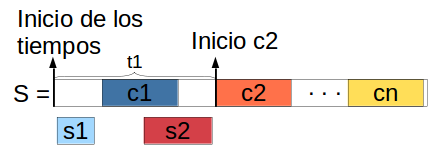
\includegraphics[scale=0.8]{ej2/Graficos/casoA.png}\\
Para que esto pase s1 debe terminar antes de c1, como nuestro algoritmo los coloca según el orden de sus finales esto es absurdo; dado que el algoritmo hubiera colocado primero a s1. \\

\textbf{Caso B:} s2 no se superpone con c1\\
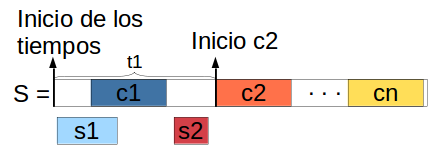
\includegraphics[scale=0.8]{ej2/Graficos/casoB.png}\\
Para que esto pase s2 debe empezar luego del final de c1, y como deben estar dentro del rango, debe terminar antes de c2. Esto es absurdo porque en este caso, al no haber conflicto ni con c1 ni con c2, el algoritmo lo hubiera colocado entremedio de estos.\\
\textit{Observación:} en este caso, el algortimo hubiese elegido s1 en vez de c1 pero esto no modifica la cantidad de cursos de S.\\

El caso en que ambos (s1 y s2) no se superponen con c1 es trivial luego de las explicaciones de los casos A y B.\\
\textit{Observación:} estos casos donde no se superponen prueban que no se puede "sacar"  0 cursos y agregar 1.\\

\newpage
\textbf{Caso C:} ambos (s1 y s2) se superponen con c1\\
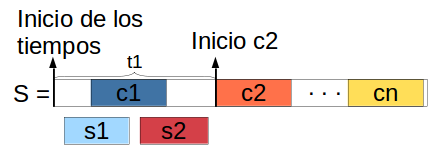
\includegraphics[scale=0.8]{ej2/Graficos/casoC.png}\\
De estas características se desprende que la única forma de que estén dispuestos s1 y s2 es que s1 finalice dentro del rango de c1 y s2 comience dentro del rango de c1.\\
Por lo tanto s1 terminaría antes que c1, es decir, nuestro algoritmo lo hubiese colocado en lugar de c1 y sería el primer curso de la solución. Entonces S no sería la solución dada por el algoritmo.\\

Por lo tanto c1 es una elección correcta y no hay forma de cambiar el curso por otros dos.\\

\textbf{Si se quiere sacar 2 cursos y agregar 3:}\\
Por la explicacion anterios sabemos que c1 está correctamente elegido, entonces la única forma de colocar 3 cursos donde antes había dos es reemplazar c2 por dos cursos. Probandolo de la misma forma que para c1 se llega a un absurdo.\\

Por lo tanto c1 y c2 son elecciones correctas y no hay forma de cambiar dos cursos por otros tres.\\

\textbf{Si se quiere sacar k cursos y agregar k+1:}\\
Extendiendolo de esa forma se llega a que no hay una manera de colocar k+1 cursos.\\

\textit{Nota:} Esto se generaliza para el caso de tomar cursos aleatorios (no sólo adyacentes) ya que la explicación es esencialmente la misma. Elegimos hacerlo en orden sólo por una cuestión de claridad.\\




%\subsection{Complejidad}
Para determinar la complejidad del algoritmo es necesario evaluar en primera instancia cuáles son las familias de casos en los cuales el algoritmo funciona peor en términos de eficiencia. Al ser una algoritmo de backtracking podado, concluimos que hallar una familia que cumpla con estas características es encontrar casos en donde las podas no tengan efecto, es decir, que no corten con las ramas de decisión tomadas. Analizándolo, determinamos que estos casos son aquellos en los cuales el algoritmo debe probar todas las combinaciones posibles y esto sucede en ejemplos como el siguiente:


\includegraphics[scale=0.5]{ej3/imgs/ajedrezDibujo.png}

Como podemos observar, el hecho de que las paredes se encuentren ubicadas de esta forma fuerzan a que las combinaciones que tenga que probar el algoritmo sean 4 por casillero porque colocar sensores en cualquier casillero libre no afecta a otros casilleros por el simple hecho de que los lasers emitidos no van a impactar en ninguno de ellos como consecuencia de las paredes. Es por esta razón que tendremos que probar $4^C$ combinaciones en donde C es la cantidad de casilleros libres.\footnote{notar que en caso de no tener podas el peor caso sería la matriz con todos casilleros libres y la complejidad se elevaría a $4^{n*m}$, donde (n*m)=tamaño de la matriz} Observando el gráfico se deduce que la cantidad de casilleros libres es la mitad de la cantidad de casilleros presentes, es decir, $(n*m)/2$.

Resumiendo, el algoritmo tendrá que realizar probar $4^{(n*m)/2}$ combinaciones en total en donde cada combinacion tiene un costo que esta determinado por complejidad de las operaciones que realizamos en cada llamada a la función Backtrack. Veamos cuál es el coste analizando el pseudocódigo:

\begin{algorithm}[H]
\caption{Backtrack}\label{Backtrack}
\begin{algorithmic}[1]
\Procedure{Backtrack}{$vector<int> casillerosUsados, int costo$}%\Comment{casillerosUsados: casilleros que fueron cubiertos hasta el momento, costo: dinero acumulado hasta el momento.}
	\State $vector<bool>\ casillerosUsadosViejo$ %\Comment{vector auxiliar para que sea posible volver a una rama anterior dentro de nuestro arbol de decisiones}
	\State $int\ aux$
	\If{$\neg hayMas(casillerosUsados)$}
		\If{$esSolucion() \wedge costo < \_costo$}
			\State $\_matrizRes=\_matriz$ % \Comment{guardo el resultado}
			\State $\_costo=costo $ %\Comment{actualizo el costo óptimo hasta el momento}
		\EndIf
	\Else
		\If{$costo<\_costo \wedge cumpleHastaElMomento(casillerosUsados)$}
			\State $casillerosUsadosViejo = casillerosUsados$ %\Comment{Guardo una copia antes de que sea modificado.}
			\ForAll{$c \in \_casilleros$}
				\If{$\neg usado(c,casillerosUsados)$}
					\ForAll{$s \in Sensores$}
						\If{$puedoColocarSensor(c,s,\_matriz)$}
							\State $InsertarSensor(c,s,\_matriz)$ 
							\State $marcarCasilleros(c,s,casillerosUsados)$
							\If{$esSensorBidireccional(s)$} 
								\State $backtrack(casillerosUsados,costo+4000)$
							\Else
								\State $backtrack(casillerosUsados,costo+6000)$
							\EndIf
							\State $sacarSensor(c,s,\_matriz)$ 
							\State $casillerosUsados=casillerosUsadosViejo$
						\EndIf
					\EndFor
					%\Comment{Caso en el que no se inserta ningún sensor.}
					\State $marcarCasillero(c,casillerosUsados)$
					\State $backtrack(casillerosUsados,costo)$
					\State $casillerosUsados=casillerosUsadosViejo$
				\EndIf
			\EndFor
		\EndIf
	\EndIf	
\EndProcedure
\end{algorithmic}
\end{algorithm}

Podemos decir que:

\begin{itemize}
	\item[1] hayMas(casillerosUsados) recorre el vector de casilleros Usados cuyo tamaño es la cantidad de casilleros simples de la grilla. Complejidad: $\mathcal{O}.((m*n)/2)$ (cantidad de casilleros de esta familia de casos)
	\item[2] esSolucion() verifica para cada uno de los casilleros simples si es apuntado por algun sensor. Verificar si es apuntado por un sensor cuesta $\mathcal{O}(1)$ ya que la función que se encarga de eso solo se mueve por la fila o columna de la matriz del casillero hasta encontrar una pared o el límite de la matriz y como mucho solo se va a mover un solo casillero. Complejidad: $\mathcal{O}((m*n)/2)$.
	\item[3] usado(c,CasillerosUsados) recorre el vector de casilleros usados. Complejidad: $\mathcal{O}((m*n)/2)$.
	\item[4] puedoColocarSensor(c,s,$\_$matriz) verifica si hay algun sensor en la columna o fila donde se va a colocar el sensor lo cual es $\mathcal{O}(1)$ ya que al igual que en el caso de esSolucion() va a moverse solo un casillero por la presencia de una pared o límite de la matriz. Complejidad: $\mathcal{O}(1)$.
	\item[5] InsertarSensor(c,s,$\_$matriz) es $\mathcal{O}(1)$ ya que simplemente se inserta en la coordenada c de la matriz un valor númerico que identifica a un laser.
	\item[6] marcarCasilleros(c,s,casillerosUsados) recorre el vector de casilleros usados. Complejidad: $\mathcal{O}((m*n)/2)$.
	\item[7] sacarSensor(c,s,$\_$matriz) es $\mathcal{O}(1)$ ya que simplemente se inserta en las coordenada c de la matriz un valor númerico.
\end{itemize}

Los items 4,5,6 y 7 se encuentran dentro de un for que recorre todos los casilleros simples por lo cual la complejidad de ese pedazo será: $\mathcal{O}((m*n)/2)$ * ($\mathcal{O}(1)$ $+$ $\mathcal{O}(1)$ $+$ $\mathcal{O}((m*n)/2)$ $+$ $\mathcal{O}(1)$ ).

Por lo tanto la complejidad de cada pasada del Backtrack es:
$\mathcal{O}((m*n)/2)$ $+$ $\mathcal{O}((m*n)/2)$ + $\mathcal{O}((m*n)/2)$ $+$ $\mathcal{O}((m*n)/2)$ * ($\mathcal{O}(1)$ $+$ $\mathcal{O}(1)$ $+$ $\mathcal{O}((m*n)/2)$ $+$ $\mathcal{O}(1)$ ) = $\mathcal{O}((m*n)/2)$ $*$ $\mathcal{O}((m*n)/2)$

En conclusión, la complejidad total del algoritmo es:

$\mathcal{O}(4^{((m*n)/2)}*((m*n)/2))^2$

%\input{ej1/codigo_relevante.tex}
%\subsection{Complejidad}
Para determinar la complejidad del algoritmo es necesario evaluar en primera instancia cuáles son las familias de casos en los cuales el algoritmo funciona peor en términos de eficiencia. Al ser una algoritmo de backtracking podado, concluimos que hallar una familia que cumpla con estas características es encontrar casos en donde las podas no tengan efecto, es decir, que no corten con las ramas de decisión tomadas. Analizándolo, determinamos que estos casos son aquellos en los cuales el algoritmo debe probar todas las combinaciones posibles y esto sucede en ejemplos como el siguiente:


\includegraphics[scale=0.5]{ej3/imgs/ajedrezDibujo.png}

Como podemos observar, el hecho de que las paredes se encuentren ubicadas de esta forma fuerzan a que las combinaciones que tenga que probar el algoritmo sean 4 por casillero porque colocar sensores en cualquier casillero libre no afecta a otros casilleros por el simple hecho de que los lasers emitidos no van a impactar en ninguno de ellos como consecuencia de las paredes. Es por esta razón que tendremos que probar $4^C$ combinaciones en donde C es la cantidad de casilleros libres.\footnote{notar que en caso de no tener podas el peor caso sería la matriz con todos casilleros libres y la complejidad se elevaría a $4^{n*m}$, donde (n*m)=tamaño de la matriz} Observando el gráfico se deduce que la cantidad de casilleros libres es la mitad de la cantidad de casilleros presentes, es decir, $(n*m)/2$.

Resumiendo, el algoritmo tendrá que realizar probar $4^{(n*m)/2}$ combinaciones en total en donde cada combinacion tiene un costo que esta determinado por complejidad de las operaciones que realizamos en cada llamada a la función Backtrack. Veamos cuál es el coste analizando el pseudocódigo:

\begin{algorithm}[H]
\caption{Backtrack}\label{Backtrack}
\begin{algorithmic}[1]
\Procedure{Backtrack}{$vector<int> casillerosUsados, int costo$}%\Comment{casillerosUsados: casilleros que fueron cubiertos hasta el momento, costo: dinero acumulado hasta el momento.}
	\State $vector<bool>\ casillerosUsadosViejo$ %\Comment{vector auxiliar para que sea posible volver a una rama anterior dentro de nuestro arbol de decisiones}
	\State $int\ aux$
	\If{$\neg hayMas(casillerosUsados)$}
		\If{$esSolucion() \wedge costo < \_costo$}
			\State $\_matrizRes=\_matriz$ % \Comment{guardo el resultado}
			\State $\_costo=costo $ %\Comment{actualizo el costo óptimo hasta el momento}
		\EndIf
	\Else
		\If{$costo<\_costo \wedge cumpleHastaElMomento(casillerosUsados)$}
			\State $casillerosUsadosViejo = casillerosUsados$ %\Comment{Guardo una copia antes de que sea modificado.}
			\ForAll{$c \in \_casilleros$}
				\If{$\neg usado(c,casillerosUsados)$}
					\ForAll{$s \in Sensores$}
						\If{$puedoColocarSensor(c,s,\_matriz)$}
							\State $InsertarSensor(c,s,\_matriz)$ 
							\State $marcarCasilleros(c,s,casillerosUsados)$
							\If{$esSensorBidireccional(s)$} 
								\State $backtrack(casillerosUsados,costo+4000)$
							\Else
								\State $backtrack(casillerosUsados,costo+6000)$
							\EndIf
							\State $sacarSensor(c,s,\_matriz)$ 
							\State $casillerosUsados=casillerosUsadosViejo$
						\EndIf
					\EndFor
					%\Comment{Caso en el que no se inserta ningún sensor.}
					\State $marcarCasillero(c,casillerosUsados)$
					\State $backtrack(casillerosUsados,costo)$
					\State $casillerosUsados=casillerosUsadosViejo$
				\EndIf
			\EndFor
		\EndIf
	\EndIf	
\EndProcedure
\end{algorithmic}
\end{algorithm}

Podemos decir que:

\begin{itemize}
	\item[1] hayMas(casillerosUsados) recorre el vector de casilleros Usados cuyo tamaño es la cantidad de casilleros simples de la grilla. Complejidad: $\mathcal{O}.((m*n)/2)$ (cantidad de casilleros de esta familia de casos)
	\item[2] esSolucion() verifica para cada uno de los casilleros simples si es apuntado por algun sensor. Verificar si es apuntado por un sensor cuesta $\mathcal{O}(1)$ ya que la función que se encarga de eso solo se mueve por la fila o columna de la matriz del casillero hasta encontrar una pared o el límite de la matriz y como mucho solo se va a mover un solo casillero. Complejidad: $\mathcal{O}((m*n)/2)$.
	\item[3] usado(c,CasillerosUsados) recorre el vector de casilleros usados. Complejidad: $\mathcal{O}((m*n)/2)$.
	\item[4] puedoColocarSensor(c,s,$\_$matriz) verifica si hay algun sensor en la columna o fila donde se va a colocar el sensor lo cual es $\mathcal{O}(1)$ ya que al igual que en el caso de esSolucion() va a moverse solo un casillero por la presencia de una pared o límite de la matriz. Complejidad: $\mathcal{O}(1)$.
	\item[5] InsertarSensor(c,s,$\_$matriz) es $\mathcal{O}(1)$ ya que simplemente se inserta en la coordenada c de la matriz un valor númerico que identifica a un laser.
	\item[6] marcarCasilleros(c,s,casillerosUsados) recorre el vector de casilleros usados. Complejidad: $\mathcal{O}((m*n)/2)$.
	\item[7] sacarSensor(c,s,$\_$matriz) es $\mathcal{O}(1)$ ya que simplemente se inserta en las coordenada c de la matriz un valor númerico.
\end{itemize}

Los items 4,5,6 y 7 se encuentran dentro de un for que recorre todos los casilleros simples por lo cual la complejidad de ese pedazo será: $\mathcal{O}((m*n)/2)$ * ($\mathcal{O}(1)$ $+$ $\mathcal{O}(1)$ $+$ $\mathcal{O}((m*n)/2)$ $+$ $\mathcal{O}(1)$ ).

Por lo tanto la complejidad de cada pasada del Backtrack es:
$\mathcal{O}((m*n)/2)$ $+$ $\mathcal{O}((m*n)/2)$ + $\mathcal{O}((m*n)/2)$ $+$ $\mathcal{O}((m*n)/2)$ * ($\mathcal{O}(1)$ $+$ $\mathcal{O}(1)$ $+$ $\mathcal{O}((m*n)/2)$ $+$ $\mathcal{O}(1)$ ) = $\mathcal{O}((m*n)/2)$ $*$ $\mathcal{O}((m*n)/2)$

En conclusión, la complejidad total del algoritmo es:

$\mathcal{O}(4^{((m*n)/2)}*((m*n)/2))^2$

%\subsection{Tests}
\textbf{Experimentos con instancias aleatorias:}\\

Para generar estas instancias utilizamos la función rand() incluida en la Standard General Utilities Library\footnote{http://www.cplusplus.com/reference/cstdlib/}. Esta función genera números pseudo-random.\\

Nuestro generador de casos requiere como datos de entrada una cantidad máxima de paquetes, luego crea casos distintos desde 1 paquete hasta la cantidad pasada de la siguiente manera:\\
Genera un peso límite al azar entre 1 y 100.\\
Para cada paquete genera un peso individual al azar entre 1 y peso límite.\\


\newpage

\section{Ejercicio 2}
%\subsection{Descripci\'on}

% Describir detalladamente el problema a resolver dando ejemplos del mismo y sus soluciones.

El sistema utilizado por Pascual consiste en cargar paquetes en camiones, de acuerdo al orden de llegada. Cada paquete se intenta cargar en el cami\'on con menor peso (con peso mayor que cero), si no es posible se guarda en un nuevo cami\'on.

El problema pide que se implemente el sistema utilizado por Pascual, con L (el peso m\'aximo soportado por todos los camiones), n (la cantidad de paquetes a cargar) y $p_1$, $p_2$, ..., $p_n$ (pesos de los paquetes) los par\'ametros de entrada.  Se supone que los paquetes no superan la capacidad m\'axima de los camiones.
Hagamos un ejemplo a modo de ilustraci\'on:

Sea L = 25, n = 7 y $p_1$ = 25, $p_2$ = 13, $p_3$ = 18, $p_4$ = 8, $p_5$ = 12, $p_6$ = 4 y $p_7$ = 1.
De acuerdo al m\'etodo del buen hombre, la soluci\'on es utilizar cuatro camiones con 25, 21, 18 y 17 sus pesos respectivos. El primer cami\'on contiene el primer paquete, el segundo cami\'on contiene al segundo y al cuarto paquete, el tercer cami\'on contiene el tercer paquete, el cuarto cami\'on contiene al quinto, sexto y s\'eptimo paquete.


\subsection{Pseudoc\'odigo}

%Explicar de forma clara, sencilla, estructurada y concisa, las ideas desarrolladas para la resolucion del problema- Para esto se sugiere utilizar pseudocodigo y lenguaje coloquial combinando adecuadamente ambas herramientas. Es importante que lo expuesto en este punto sea suficiente para el desarrollo de los puntos subsiguientes, pero no excesivo.



%\subsection{Demostraci\'on}

Sea S una solución dada por nuestro algoritmo, supongo que existe S* tal que tiene al menos un curso más que S. Es lo mismo que decir que podemos sacar k cursos de S y agregar, como mínimo, k$+$1 (con 0$<$k$\leq$n, n=$\#$S).\\

\textbf{Si se quiere sacar un curso y agregar dos:}\\
Supongo que podemos sacar el primer curso (c1) de S y poner dos en su lugar. Para que dos cursos (s1, s2) quepan en el tiempo que quedó libre (t1) tienen que cumplir las siguientes características:
\begin{enumerate}
\item No se deben solapar entre sí (sino no podrían agregarse juntos).
\item Sus inicios y fines deben estar dentro del rango de tiempo libre (t1).
\end{enumerate}
Con esto lo podemos dividir en casos:\\

\textbf{Caso A:} s1 no se superpone con c1\\
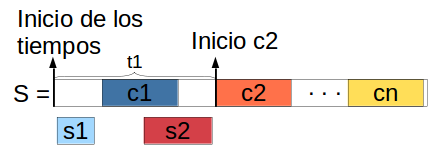
\includegraphics[scale=0.8]{ej2/Graficos/casoA.png}\\
Para que esto pase s1 debe terminar antes de c1, como nuestro algoritmo los coloca según el orden de sus finales esto es absurdo; dado que el algoritmo hubiera colocado primero a s1. \\

\textbf{Caso B:} s2 no se superpone con c1\\
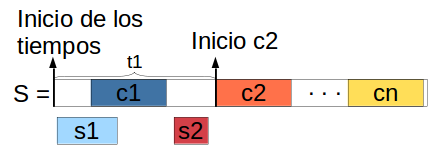
\includegraphics[scale=0.8]{ej2/Graficos/casoB.png}\\
Para que esto pase s2 debe empezar luego del final de c1, y como deben estar dentro del rango, debe terminar antes de c2. Esto es absurdo porque en este caso, al no haber conflicto ni con c1 ni con c2, el algoritmo lo hubiera colocado entremedio de estos.\\
\textit{Observación:} en este caso, el algortimo hubiese elegido s1 en vez de c1 pero esto no modifica la cantidad de cursos de S.\\

El caso en que ambos (s1 y s2) no se superponen con c1 es trivial luego de las explicaciones de los casos A y B.\\
\textit{Observación:} estos casos donde no se superponen prueban que no se puede "sacar"  0 cursos y agregar 1.\\

\newpage
\textbf{Caso C:} ambos (s1 y s2) se superponen con c1\\
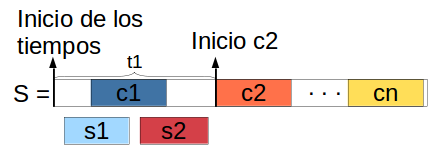
\includegraphics[scale=0.8]{ej2/Graficos/casoC.png}\\
De estas características se desprende que la única forma de que estén dispuestos s1 y s2 es que s1 finalice dentro del rango de c1 y s2 comience dentro del rango de c1.\\
Por lo tanto s1 terminaría antes que c1, es decir, nuestro algoritmo lo hubiese colocado en lugar de c1 y sería el primer curso de la solución. Entonces S no sería la solución dada por el algoritmo.\\

Por lo tanto c1 es una elección correcta y no hay forma de cambiar el curso por otros dos.\\

\textbf{Si se quiere sacar 2 cursos y agregar 3:}\\
Por la explicacion anterios sabemos que c1 está correctamente elegido, entonces la única forma de colocar 3 cursos donde antes había dos es reemplazar c2 por dos cursos. Probandolo de la misma forma que para c1 se llega a un absurdo.\\

Por lo tanto c1 y c2 son elecciones correctas y no hay forma de cambiar dos cursos por otros tres.\\

\textbf{Si se quiere sacar k cursos y agregar k+1:}\\
Extendiendolo de esa forma se llega a que no hay una manera de colocar k+1 cursos.\\

\textit{Nota:} Esto se generaliza para el caso de tomar cursos aleatorios (no sólo adyacentes) ya que la explicación es esencialmente la misma. Elegimos hacerlo en orden sólo por una cuestión de claridad.\\




%\subsection{Complejidad}
Para determinar la complejidad del algoritmo es necesario evaluar en primera instancia cuáles son las familias de casos en los cuales el algoritmo funciona peor en términos de eficiencia. Al ser una algoritmo de backtracking podado, concluimos que hallar una familia que cumpla con estas características es encontrar casos en donde las podas no tengan efecto, es decir, que no corten con las ramas de decisión tomadas. Analizándolo, determinamos que estos casos son aquellos en los cuales el algoritmo debe probar todas las combinaciones posibles y esto sucede en ejemplos como el siguiente:


\includegraphics[scale=0.5]{ej3/imgs/ajedrezDibujo.png}

Como podemos observar, el hecho de que las paredes se encuentren ubicadas de esta forma fuerzan a que las combinaciones que tenga que probar el algoritmo sean 4 por casillero porque colocar sensores en cualquier casillero libre no afecta a otros casilleros por el simple hecho de que los lasers emitidos no van a impactar en ninguno de ellos como consecuencia de las paredes. Es por esta razón que tendremos que probar $4^C$ combinaciones en donde C es la cantidad de casilleros libres.\footnote{notar que en caso de no tener podas el peor caso sería la matriz con todos casilleros libres y la complejidad se elevaría a $4^{n*m}$, donde (n*m)=tamaño de la matriz} Observando el gráfico se deduce que la cantidad de casilleros libres es la mitad de la cantidad de casilleros presentes, es decir, $(n*m)/2$.

Resumiendo, el algoritmo tendrá que realizar probar $4^{(n*m)/2}$ combinaciones en total en donde cada combinacion tiene un costo que esta determinado por complejidad de las operaciones que realizamos en cada llamada a la función Backtrack. Veamos cuál es el coste analizando el pseudocódigo:

\begin{algorithm}[H]
\caption{Backtrack}\label{Backtrack}
\begin{algorithmic}[1]
\Procedure{Backtrack}{$vector<int> casillerosUsados, int costo$}%\Comment{casillerosUsados: casilleros que fueron cubiertos hasta el momento, costo: dinero acumulado hasta el momento.}
	\State $vector<bool>\ casillerosUsadosViejo$ %\Comment{vector auxiliar para que sea posible volver a una rama anterior dentro de nuestro arbol de decisiones}
	\State $int\ aux$
	\If{$\neg hayMas(casillerosUsados)$}
		\If{$esSolucion() \wedge costo < \_costo$}
			\State $\_matrizRes=\_matriz$ % \Comment{guardo el resultado}
			\State $\_costo=costo $ %\Comment{actualizo el costo óptimo hasta el momento}
		\EndIf
	\Else
		\If{$costo<\_costo \wedge cumpleHastaElMomento(casillerosUsados)$}
			\State $casillerosUsadosViejo = casillerosUsados$ %\Comment{Guardo una copia antes de que sea modificado.}
			\ForAll{$c \in \_casilleros$}
				\If{$\neg usado(c,casillerosUsados)$}
					\ForAll{$s \in Sensores$}
						\If{$puedoColocarSensor(c,s,\_matriz)$}
							\State $InsertarSensor(c,s,\_matriz)$ 
							\State $marcarCasilleros(c,s,casillerosUsados)$
							\If{$esSensorBidireccional(s)$} 
								\State $backtrack(casillerosUsados,costo+4000)$
							\Else
								\State $backtrack(casillerosUsados,costo+6000)$
							\EndIf
							\State $sacarSensor(c,s,\_matriz)$ 
							\State $casillerosUsados=casillerosUsadosViejo$
						\EndIf
					\EndFor
					%\Comment{Caso en el que no se inserta ningún sensor.}
					\State $marcarCasillero(c,casillerosUsados)$
					\State $backtrack(casillerosUsados,costo)$
					\State $casillerosUsados=casillerosUsadosViejo$
				\EndIf
			\EndFor
		\EndIf
	\EndIf	
\EndProcedure
\end{algorithmic}
\end{algorithm}

Podemos decir que:

\begin{itemize}
	\item[1] hayMas(casillerosUsados) recorre el vector de casilleros Usados cuyo tamaño es la cantidad de casilleros simples de la grilla. Complejidad: $\mathcal{O}.((m*n)/2)$ (cantidad de casilleros de esta familia de casos)
	\item[2] esSolucion() verifica para cada uno de los casilleros simples si es apuntado por algun sensor. Verificar si es apuntado por un sensor cuesta $\mathcal{O}(1)$ ya que la función que se encarga de eso solo se mueve por la fila o columna de la matriz del casillero hasta encontrar una pared o el límite de la matriz y como mucho solo se va a mover un solo casillero. Complejidad: $\mathcal{O}((m*n)/2)$.
	\item[3] usado(c,CasillerosUsados) recorre el vector de casilleros usados. Complejidad: $\mathcal{O}((m*n)/2)$.
	\item[4] puedoColocarSensor(c,s,$\_$matriz) verifica si hay algun sensor en la columna o fila donde se va a colocar el sensor lo cual es $\mathcal{O}(1)$ ya que al igual que en el caso de esSolucion() va a moverse solo un casillero por la presencia de una pared o límite de la matriz. Complejidad: $\mathcal{O}(1)$.
	\item[5] InsertarSensor(c,s,$\_$matriz) es $\mathcal{O}(1)$ ya que simplemente se inserta en la coordenada c de la matriz un valor númerico que identifica a un laser.
	\item[6] marcarCasilleros(c,s,casillerosUsados) recorre el vector de casilleros usados. Complejidad: $\mathcal{O}((m*n)/2)$.
	\item[7] sacarSensor(c,s,$\_$matriz) es $\mathcal{O}(1)$ ya que simplemente se inserta en las coordenada c de la matriz un valor númerico.
\end{itemize}

Los items 4,5,6 y 7 se encuentran dentro de un for que recorre todos los casilleros simples por lo cual la complejidad de ese pedazo será: $\mathcal{O}((m*n)/2)$ * ($\mathcal{O}(1)$ $+$ $\mathcal{O}(1)$ $+$ $\mathcal{O}((m*n)/2)$ $+$ $\mathcal{O}(1)$ ).

Por lo tanto la complejidad de cada pasada del Backtrack es:
$\mathcal{O}((m*n)/2)$ $+$ $\mathcal{O}((m*n)/2)$ + $\mathcal{O}((m*n)/2)$ $+$ $\mathcal{O}((m*n)/2)$ * ($\mathcal{O}(1)$ $+$ $\mathcal{O}(1)$ $+$ $\mathcal{O}((m*n)/2)$ $+$ $\mathcal{O}(1)$ ) = $\mathcal{O}((m*n)/2)$ $*$ $\mathcal{O}((m*n)/2)$

En conclusión, la complejidad total del algoritmo es:

$\mathcal{O}(4^{((m*n)/2)}*((m*n)/2))^2$

%\input{ej2/codigo_relevante.tex}
%\subsection{Complejidad}
Para determinar la complejidad del algoritmo es necesario evaluar en primera instancia cuáles son las familias de casos en los cuales el algoritmo funciona peor en términos de eficiencia. Al ser una algoritmo de backtracking podado, concluimos que hallar una familia que cumpla con estas características es encontrar casos en donde las podas no tengan efecto, es decir, que no corten con las ramas de decisión tomadas. Analizándolo, determinamos que estos casos son aquellos en los cuales el algoritmo debe probar todas las combinaciones posibles y esto sucede en ejemplos como el siguiente:


\includegraphics[scale=0.5]{ej3/imgs/ajedrezDibujo.png}

Como podemos observar, el hecho de que las paredes se encuentren ubicadas de esta forma fuerzan a que las combinaciones que tenga que probar el algoritmo sean 4 por casillero porque colocar sensores en cualquier casillero libre no afecta a otros casilleros por el simple hecho de que los lasers emitidos no van a impactar en ninguno de ellos como consecuencia de las paredes. Es por esta razón que tendremos que probar $4^C$ combinaciones en donde C es la cantidad de casilleros libres.\footnote{notar que en caso de no tener podas el peor caso sería la matriz con todos casilleros libres y la complejidad se elevaría a $4^{n*m}$, donde (n*m)=tamaño de la matriz} Observando el gráfico se deduce que la cantidad de casilleros libres es la mitad de la cantidad de casilleros presentes, es decir, $(n*m)/2$.

Resumiendo, el algoritmo tendrá que realizar probar $4^{(n*m)/2}$ combinaciones en total en donde cada combinacion tiene un costo que esta determinado por complejidad de las operaciones que realizamos en cada llamada a la función Backtrack. Veamos cuál es el coste analizando el pseudocódigo:

\begin{algorithm}[H]
\caption{Backtrack}\label{Backtrack}
\begin{algorithmic}[1]
\Procedure{Backtrack}{$vector<int> casillerosUsados, int costo$}%\Comment{casillerosUsados: casilleros que fueron cubiertos hasta el momento, costo: dinero acumulado hasta el momento.}
	\State $vector<bool>\ casillerosUsadosViejo$ %\Comment{vector auxiliar para que sea posible volver a una rama anterior dentro de nuestro arbol de decisiones}
	\State $int\ aux$
	\If{$\neg hayMas(casillerosUsados)$}
		\If{$esSolucion() \wedge costo < \_costo$}
			\State $\_matrizRes=\_matriz$ % \Comment{guardo el resultado}
			\State $\_costo=costo $ %\Comment{actualizo el costo óptimo hasta el momento}
		\EndIf
	\Else
		\If{$costo<\_costo \wedge cumpleHastaElMomento(casillerosUsados)$}
			\State $casillerosUsadosViejo = casillerosUsados$ %\Comment{Guardo una copia antes de que sea modificado.}
			\ForAll{$c \in \_casilleros$}
				\If{$\neg usado(c,casillerosUsados)$}
					\ForAll{$s \in Sensores$}
						\If{$puedoColocarSensor(c,s,\_matriz)$}
							\State $InsertarSensor(c,s,\_matriz)$ 
							\State $marcarCasilleros(c,s,casillerosUsados)$
							\If{$esSensorBidireccional(s)$} 
								\State $backtrack(casillerosUsados,costo+4000)$
							\Else
								\State $backtrack(casillerosUsados,costo+6000)$
							\EndIf
							\State $sacarSensor(c,s,\_matriz)$ 
							\State $casillerosUsados=casillerosUsadosViejo$
						\EndIf
					\EndFor
					%\Comment{Caso en el que no se inserta ningún sensor.}
					\State $marcarCasillero(c,casillerosUsados)$
					\State $backtrack(casillerosUsados,costo)$
					\State $casillerosUsados=casillerosUsadosViejo$
				\EndIf
			\EndFor
		\EndIf
	\EndIf	
\EndProcedure
\end{algorithmic}
\end{algorithm}

Podemos decir que:

\begin{itemize}
	\item[1] hayMas(casillerosUsados) recorre el vector de casilleros Usados cuyo tamaño es la cantidad de casilleros simples de la grilla. Complejidad: $\mathcal{O}.((m*n)/2)$ (cantidad de casilleros de esta familia de casos)
	\item[2] esSolucion() verifica para cada uno de los casilleros simples si es apuntado por algun sensor. Verificar si es apuntado por un sensor cuesta $\mathcal{O}(1)$ ya que la función que se encarga de eso solo se mueve por la fila o columna de la matriz del casillero hasta encontrar una pared o el límite de la matriz y como mucho solo se va a mover un solo casillero. Complejidad: $\mathcal{O}((m*n)/2)$.
	\item[3] usado(c,CasillerosUsados) recorre el vector de casilleros usados. Complejidad: $\mathcal{O}((m*n)/2)$.
	\item[4] puedoColocarSensor(c,s,$\_$matriz) verifica si hay algun sensor en la columna o fila donde se va a colocar el sensor lo cual es $\mathcal{O}(1)$ ya que al igual que en el caso de esSolucion() va a moverse solo un casillero por la presencia de una pared o límite de la matriz. Complejidad: $\mathcal{O}(1)$.
	\item[5] InsertarSensor(c,s,$\_$matriz) es $\mathcal{O}(1)$ ya que simplemente se inserta en la coordenada c de la matriz un valor númerico que identifica a un laser.
	\item[6] marcarCasilleros(c,s,casillerosUsados) recorre el vector de casilleros usados. Complejidad: $\mathcal{O}((m*n)/2)$.
	\item[7] sacarSensor(c,s,$\_$matriz) es $\mathcal{O}(1)$ ya que simplemente se inserta en las coordenada c de la matriz un valor númerico.
\end{itemize}

Los items 4,5,6 y 7 se encuentran dentro de un for que recorre todos los casilleros simples por lo cual la complejidad de ese pedazo será: $\mathcal{O}((m*n)/2)$ * ($\mathcal{O}(1)$ $+$ $\mathcal{O}(1)$ $+$ $\mathcal{O}((m*n)/2)$ $+$ $\mathcal{O}(1)$ ).

Por lo tanto la complejidad de cada pasada del Backtrack es:
$\mathcal{O}((m*n)/2)$ $+$ $\mathcal{O}((m*n)/2)$ + $\mathcal{O}((m*n)/2)$ $+$ $\mathcal{O}((m*n)/2)$ * ($\mathcal{O}(1)$ $+$ $\mathcal{O}(1)$ $+$ $\mathcal{O}((m*n)/2)$ $+$ $\mathcal{O}(1)$ ) = $\mathcal{O}((m*n)/2)$ $*$ $\mathcal{O}((m*n)/2)$

En conclusión, la complejidad total del algoritmo es:

$\mathcal{O}(4^{((m*n)/2)}*((m*n)/2))^2$

%\subsection{Tests}
\textbf{Experimentos con instancias aleatorias:}\\

Para generar estas instancias utilizamos la función rand() incluida en la Standard General Utilities Library\footnote{http://www.cplusplus.com/reference/cstdlib/}. Esta función genera números pseudo-random.\\

Nuestro generador de casos requiere como datos de entrada una cantidad máxima de paquetes, luego crea casos distintos desde 1 paquete hasta la cantidad pasada de la siguiente manera:\\
Genera un peso límite al azar entre 1 y 100.\\
Para cada paquete genera un peso individual al azar entre 1 y peso límite.\\



\end{document}
